\documentclass[14pt,UTF-8]{beamer}
\usepackage[utf8]{inputenc}
\usepackage[T1]{fontenc}
\usepackage{ctex}
\usepackage{lmodern}
%\usepackage{caption}
\usepackage{graphicx}
\usepackage{enumerate}
\usetheme{Bergen}
\begin{document}
	\author{宋振华、陈宇翔}
	\title{Linux 0.11可视化}
	\subtitle{操作系统课程设计}
	%\logo{}
	\institute{泰山学堂2016级计算机}
	\date{2018-12-25}
	%\subject{hh}
	%\setbeamercovered{transparent}
	%\setbeamertemplate{navigation symbols}{}
	\begin{frame}[plain]
	\maketitle
\end{frame}

\begin{frame}
\frametitle{阅读代码}
\begin{itemize}
	\item 总结出每个文件、每个函数的功能
	\item 绘制思维导图
\end{itemize}
\begin{figure}
	\centering
	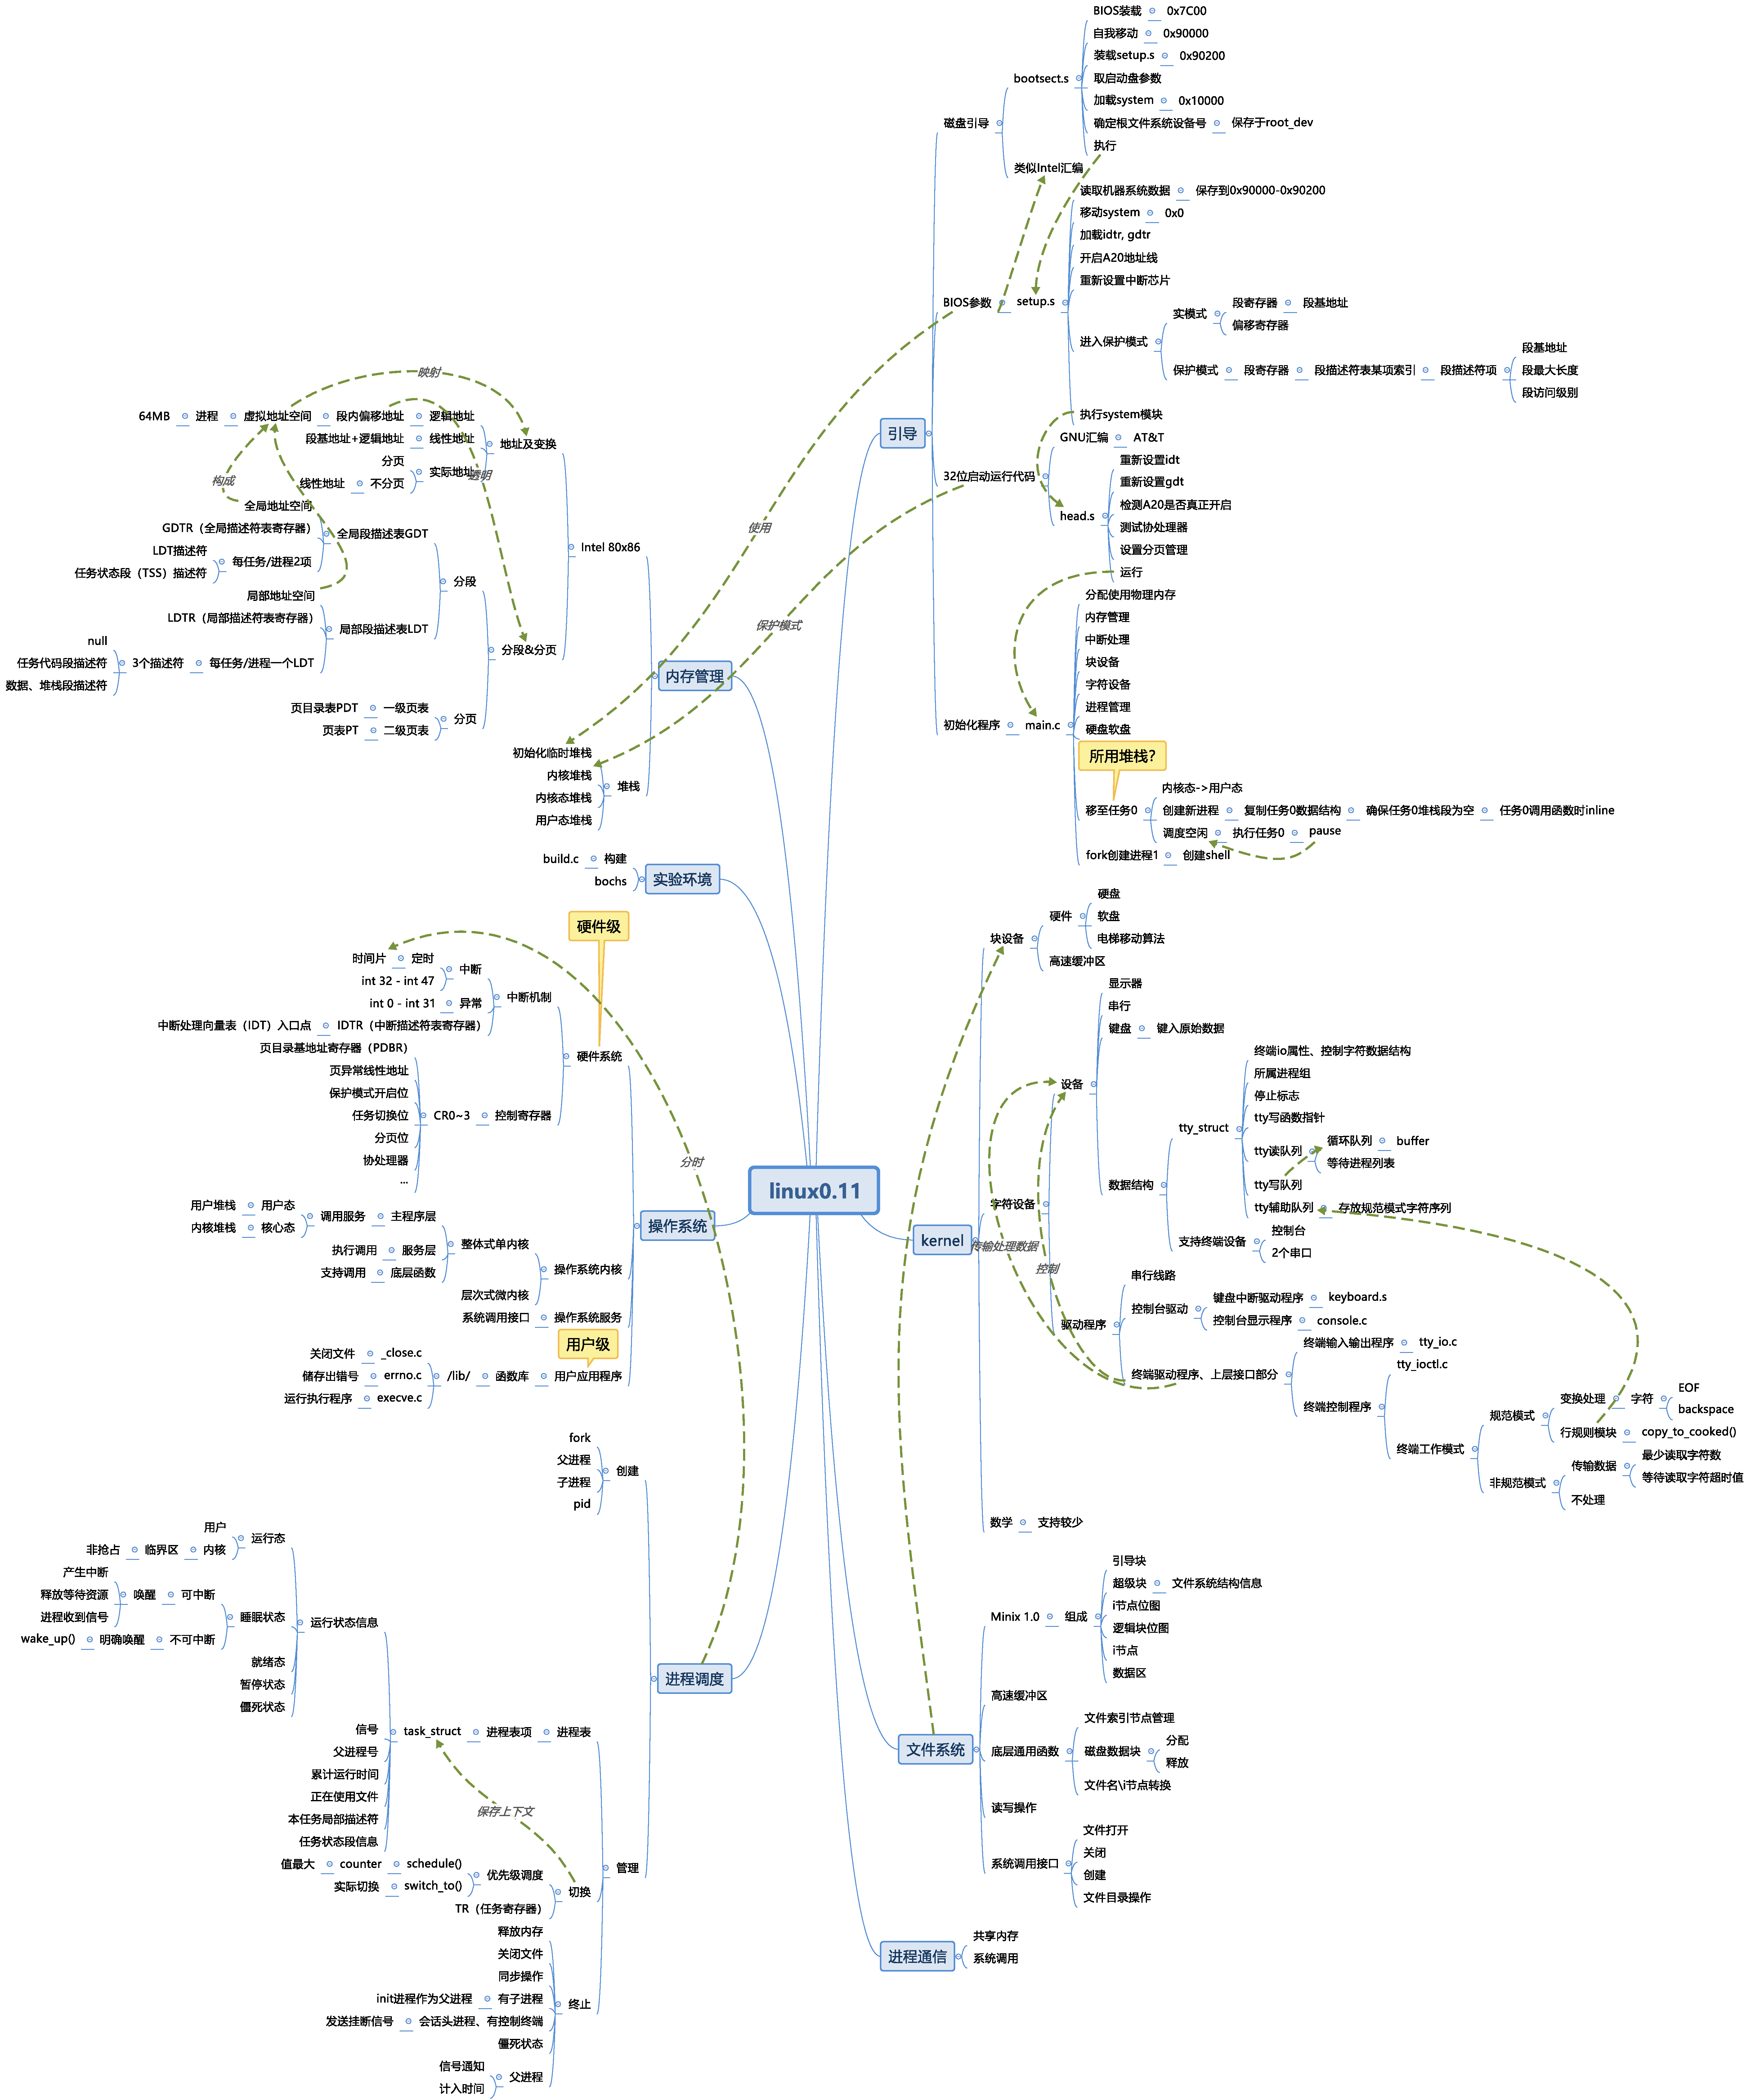
\includegraphics[width=0.6\textwidth,natwidth=2722 ,natheight=3249]{img/linux0.11.pdf}
	\label{fig:linuxgraph}
\end{figure}
\end{frame}

\begin{frame}
\frametitle{选择可视化模块}
\begin{itemize}
	\item \textbf{开机启动过程}
	
	开机启动过程中, 所有C语言函数被调用的情况
	\item \textbf{字符显示过程}
	
	控制台输入echo hello系统的执行情况;
	
	控制台输入a.out系统的执行情况;
\end{itemize}
\end{frame}


\begin{frame}
\frametitle{可视化方案}
\begin{itemize}
	\item 编程语言: HTML5+CSS3+JavaScript
	\item 开机过程用条形统计图
	\item 开机后, 使用一个动态跳动指针
	\item 访问 123.207.166.164:23333 以查看
\end{itemize}

\end{frame}

\begin{frame}
\frametitle{可视化}
\begin{figure}[htbp]
	\centering
	\includegraphics[width=\textwidth,natwidth=773 ,natheight=487]{img/index.html.pdf}
	\caption[]{主页, 包含对每个文件功能的介绍; 模拟内存及console}
	\label{fig:indexgraph}
\end{figure}
\end{frame}

\begin{frame}
\frametitle{可视化}
\begin{figure}[htbp]
	\centering
	\includegraphics[width=\textwidth,natwidth=594 ,natheight=419]{img/calledMaxFunc.pdf}
	\caption[]{“引导界面调用次数最多”的函数 统计图. 表格与条形图可进行简单的交互. 纵坐标为log坐标轴}
	\label{fig:calledMaxFuncgraph}
\end{figure}
\end{frame}

\begin{frame}
\frametitle{可视化}
\begin{figure}[htbp]
	\centering
	\includegraphics[width=\textwidth,natwidth=577 ,natheight=416]{img/calledFile.pdf}
	\caption[]{“引导界面调用次数最多”的文件 统计图}
	\label{fig:calledMaxFilegraph}
\end{figure}
\end{frame}

\begin{frame}
\frametitle{可视化}
\begin{figure}[htbp]
	\centering
	\includegraphics[width=\textwidth,natwidth=590 ,natheight=406]{img/eachFileCall.pdf}
	\caption[]{这是sched.c中函数统计调用图. 点击某函数, 可显示对应的调用字.}
	\label{fig:eachFileCallgraph}
\end{figure}
\end{frame}

\begin{frame}
\frametitle{可视化}
\begin{figure}[htbp]
	\centering
	\includegraphics[width=\textwidth,natwidth=756 ,natheight=450]{img/chrdrv.pdf}
	\caption[]{字符设备动图}
	\label{fig:ChrDrvgraph}
\end{figure}

\end{frame}
\begin{frame}
\frametitle{提取数据的方式}
\begin{itemize}
	\item \textbf{使用gdb脚本输出运行信息}
	
	支持在开机后调用某一系统调用, 以输出gdb脚本运行信息
	\item \textbf{gdb单步调试}

	用于确定断点所在位置
\end{itemize}
\end{frame}

\begin{frame}
\frametitle{感想}
\begin{enumerate}
	\item 对Linux 0.11代码有了进一步认识
	\item 对gdb脚本有了进一步认识
	\item 加强了合作、交流能力
	\item 网页制作水平得到提高
	\item 感谢杨老师一年来的教导
\end{enumerate}
\end{frame}


\end{document}